\section{First Exercise}
\subsection{Proton Collisions at the LHC}
\paragraph{a)} We have that 
\begin{equation}
	\SI{1}{\joule} = \SI{1.6e-19}{\electronvolt} = \SI{0.239}{cal},
\end{equation}
thus the conversion from eV to calories are
\begin{equation}
	\SI{1}{\electronvolt} = \SI{3.82e-20}{cal},
\end{equation}
which means that $\SI{13e12}{\electronvolt} = \SI{4.97e-6}{cal} = \SI{4.97e-10}{kcal}$

\paragraph{b)} The number of Wasa crackers in one pp collision at the LHC is 
\begin{equation}
	\frac{\SI{4.97e-10}{kcal}}{\SI{60}{kcal}} = \SI{8.28e-12}{},
\end{equation}
so only \SI{0.00000000083}{\percent} of a Wasa cracker is needed to equate the energy of one pp collision at the LHC.

\paragraph{c)} Though it seems like very little energy the particles are very small and not especially massive it is, on the particle scale, very powerful. For example, the mass of a proton is less than 1 GeV, thus the momentum in the collision is much greater than the masses involved.

\subsection{Decay of \texorpdfstring{$\pi^0$}{pi}}
\paragraph{a)} Since the pion is at rest and the photons are massless, all of the pions mass energy will be turned into kinetic energy for he photons, equally split between them to conserve momentum. Therefore $E_\gamma = \SI{67.5}{MeV}$. The momentum is $p = E/c$ and since we set $c=1$ we get that $p_\gamma = \SI{67.5}{MeV}$, and the photons have opposite direction of their momentum due to conservation of momentum.

\paragraph{b)} The total energy before the collision is then $E_\pi = m_\pi + KE_\pi = \SI{635}{MeV}$, and after the collision we therefore must have $E_{\gamma 1} + E_{\gamma 2} = E_\pi = \SI{635}{MeV}$. We have the equation
\begin{equation}
	E^2 - p^2 = m^2,
\end{equation}
which is lorentz invariant, so this can be used to calculate the momentum before the collision.
\begin{equation}
	p_\pi = \sqrt{E_\pi^2 - m_\pi^2} = \SI{620.48}{MeV}.
\end{equation}
For the photons we have that $p_\gamma = E_\gamma$, and the conservation of momentum tells us that $\vec{p}_{\gamma 1} + \vec{p}_{\gamma 2} = \vec{p}_\pi$. Setting $\vec{p}_\pi$ to be in the $x$-direction, we can split $\vec{p}_{\gamma} = p_{\gamma}^x \hat{x} + p_{\gamma}^y \hat{y}$ which gives $p_\gamma^2 = (p_\gamma^x)^2 + (p_\gamma^y)^2$. Since the decay is symmetric we know that $p_\gamma = E_\gamma = E_\pi /2 $ and $p_\gamma^x = p_\pi /2$ which gives $p_\gamma^y = \SI{67.51}{MeV}$. Then we find the angle with 
\begin{equation}
	\theta = \arctan{\frac{p_\gamma^y}{p_\gamma^x}} = 12.3^\circ
\end{equation}

\subsection{Feynman diagrams of \texorpdfstring{$\pi^0$}{pi} decay}

\begin{figure}[H]
	\centering
	\begin{subfigure}[t]{0.45\textwidth}
		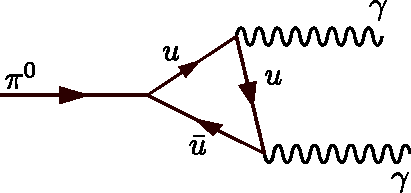
\includegraphics[width=\textwidth]{figures/feynman_a.pdf}
		\caption{The most probable decay with a \SI{98.8}{\percent} probability}
	\end{subfigure}
	\hfill
	\begin{subfigure}[t]{0.45\textwidth}
		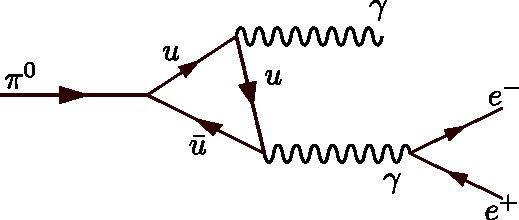
\includegraphics[width=\textwidth]{figures/feynman_b.pdf}
		\caption{The second most probable decay with a \SI{1.2}{\percent} probability}
	\end{subfigure}
	\hfill
	\begin{subfigure}[t]{0.45\textwidth}
		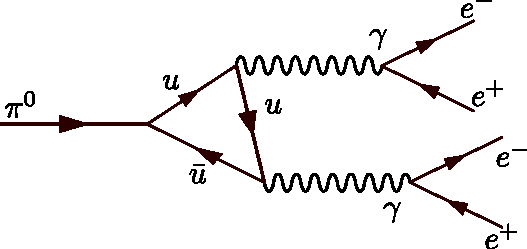
\includegraphics[width=\textwidth]{figures/feynman_c.pdf}
		\caption{The third most probable decay with a \SI{0.0031}{\percent} probability}
	\end{subfigure}
	\caption{Feynman diagrams of the different possible decays of a $\pi^0$}
\end{figure}

In a) there are two electromagnetic vertices and thus $p_a = \abs{g}^2 \propto \alpha^2$, in b) there are three electromagnetic vertices and thus $p_b = 2\abs{g}^2 \propto 2\alpha^3$ the 2 is due to that there are two possibilities for which photon decays, and in c) there are four electromagnetic vertices and thus $p\abs{g}^2 \propto \alpha^4$. The sum of all should equal $\SI{100}{\percent}$, thus
\begin{equation}
	1 = p_a + p_b + p_c = \lambda\alpha^2 + 2\lambda\alpha^3 + \lambda\alpha^4,
\end{equation}
where $\lambda$ is the proportionality constant.


Calculating $\lambda$ with $\alpha = 1/137$ we get 
\begin{equation}
	\lambda = \frac{1}{\alpha^2 + 2\alpha^3 + \alpha^4} = 18497.97,
\end{equation}
now we get the probabilities as 
\begin{align}
	p_a &= \lambda\alpha^2 = \SI{98.6}{\percent}\\
	p_b &= 2\lambda\alpha^3 = \SI[]{1.4}{\percent}\\
	p_c &= \lambda\alpha^4 = \SI[]{0.0053}{\percent}.
\end{align}
The values differ a bit from the values given in the exercise. This is probably due to the fact that $\alpha$ is not exactly equal to 137.

\subsection{Concepts in Particle Physics}
\paragraph{a)} The main experimental evidences of colour. One of them is that the ratio between crossections of electron-positron annihilation outcomes. Namely $e^+ e^- \to \mu^+ \mu^-$ and $e^+ e^- \to q \bar{q}$. The ratio $\sigma(e^+ e^- \to q \bar{q})/\sigma(e^+ e^- \to \mu^+ \mu^-) = 3$. Thus indicating that there must be three possible states for a given quark. These states are referred to as the colour of the quark. 

\paragraph{b)} The theoretical evidence is the $\Omega^-$ baryon. The quark composition is $\Omega^- = s_\uparrow s_\uparrow s_\uparrow$, with total spin $s = 3/2$ and it is thus a fermion, so the total wavefunction must be symmetric. However, the space wavefunction, flavour wavefunction, and spin wavefunction are all symmetric for this composition, therefore we must have another, antisymmetric wavefunction and we call that wavefunction for the colour wavefunction.

\paragraph{c)} A jet is a collimated stream of hadrons which is created from highly energetic quarks after high energy particle collision. The quarks release energy in form of gluons which then create quark-antiquark pairs and thus creating hadrons.

\paragraph{d)} The top quark is very heavy at $\SI[]{173}{GeV}$ which is about 183 times the mass of the proton. Since it is so heavy it decays extremely fast due to the weak interaction, which means that the top quark generally cannot create any hadrons since its half life is shorter than the timescale for gluon's hadron creation.

\subsection{Classifying Reactions}
\paragraph{a)} Both lepton number and charge is conserved in the reaction. Since the left hand side is not charged we must have a weak interaction with a $Z^0$ boson.

\begin{figure}[H]
	\centering
	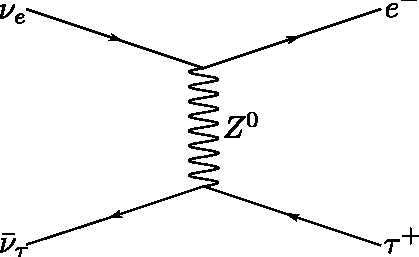
\includegraphics[width=0.5\textwidth]{figures/classify_a.pdf}
	\caption{Feynman diagram showing $\nu_e + \bar{\nu}_\tau \to e^- + \tau^+$}
\end{figure}

\paragraph{b)} Lepton and baryon number, and charge is conserved. Since we move a charge from the muon to one of the up quarks we have weak interaction with a $W^{\pm}$

\begin{figure}[H]
	\centering
	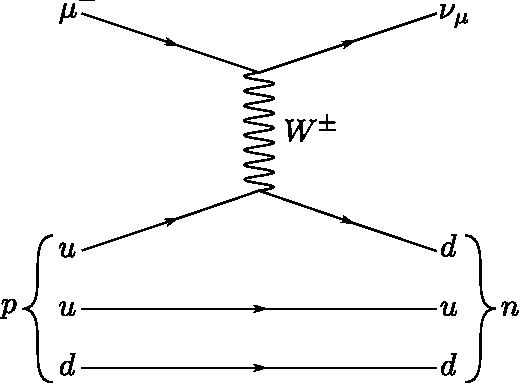
\includegraphics[width=0.5\textwidth]{figures/classify_b.pdf}
	\caption{Feynman diagram showing $\mu^- + p \to \nu_\mu + n$}
\end{figure}

\paragraph{c)} Lepton and baryon number, and charge is conserved. Since the strange is coupled to the anti-down it is a low probability weak interaction with a $W^\pm$ boson to transport charge to the muon.

\begin{figure}[H]
	\centering
	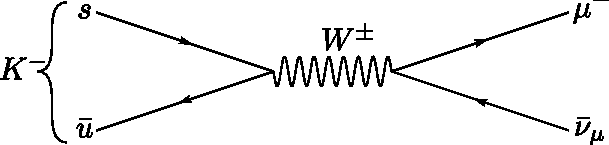
\includegraphics[width=0.5\textwidth]{figures/classify_c.pdf}
	\caption{Feynman diagram showing $K^- \to \mu^- \nu_\mu $}
\end{figure}

\paragraph{d)} Lepton number is not conserved so it is impossible.

\paragraph{e)} Lepton and baryon number, and charge is conserved. Strangeness is not conserved, and thus must decay via the weak interaction with a $W^\pm$ boson.

\begin{figure}[H]
	\centering
	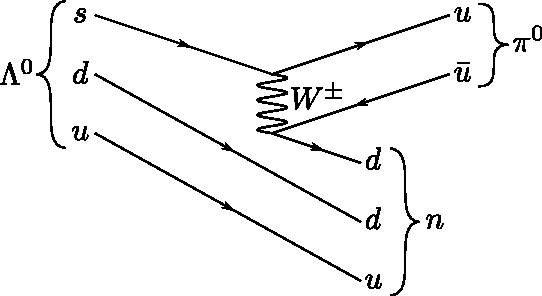
\includegraphics[width=0.5\textwidth]{figures/classify_e.pdf}
	\caption{Feynman diagram showing $\Lambda^0 \to \pi^0 + n $}
\end{figure}

\paragraph{f)} Baryon number and charge is conserved. The most probable reaction is with the strong force.

\begin{figure}[H]
	\centering
	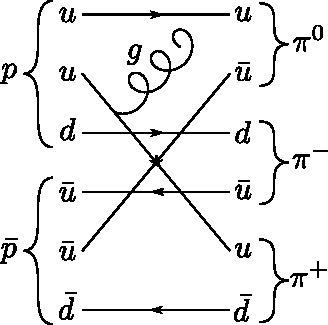
\includegraphics[width=0.5\textwidth]{figures/classify_f.pdf}
	\caption{Feynman diagram showing $p + \bar{p} \to \pi^+ + \pi^- + \pi^0 $}
\end{figure}

\paragraph{g)} Lepton and baryon number, and charge is conserved. The interaction is between charged particles so it is the electromagnetic interaction since it is stronger than the weak interaction.

\begin{figure}[H]
	\centering
	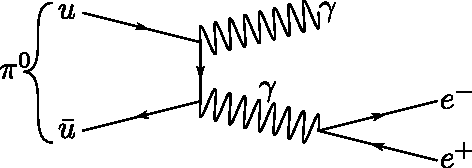
\includegraphics[width=0.5\textwidth]{figures/classify_g.pdf}
	\caption{Feynman diagram showing $\pi^0 \to \gamma + e^+ + e^- $}
\end{figure}

\paragraph{h)} Lepton and baryon number, and charge and strangeness is conserved. The quark composition is the same for $\Lambda^0$ and $\Sigma^0$ it is only the isospin that differs. The interaction is electromagnetic.

\begin{figure}[H]
	\centering
	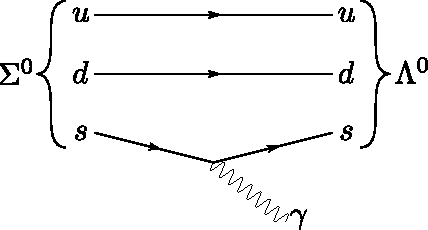
\includegraphics[width=0.5\textwidth]{figures/classify_h.pdf}
	\caption{Feynman diagram showing $\Sigma^0 \to \Lambda^0 + \gamma $}
\end{figure}

\paragraph{i)} There is no conservation of lepton number so it is impossible.